\chapter{Auswertung}

Im folgenden Kapitel wird die Auswertung anhand der in Kapitel (X) aufgestellten Bewertungskriterien beschrieben. Zu den einzelnen Kategorien (siehe Kapitel (X)) wird der jeweilige ausgefüllte Abschnitt der Bewertungsmatrix dargestellt und erläutert. 

\section{Kosten und Lizenz}

Nachfolgende Abbildung (X) zeigt den Abschnitt 'Kosten und Lizenz' der ausgefüllten Bewertungsmatrix.

\begin{figure}[h]
	\centering
	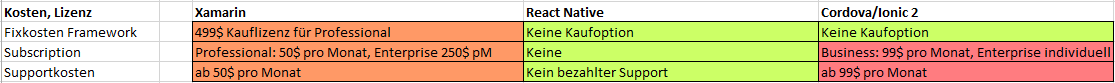
\includegraphics[width=1\textwidth]{Bilder/Auswertung_KostenLizenz.PNG}
	\caption{Bewertungsmatrix Kategorie Kosten und Lizenz}
	\label{fig:AuswKostLiz}
\end{figure}

Das Xamarin Framework gibt es in einer kostenlosen Community-Version und in den kostenpflichtigen Versionen 'Professional' und 'Enterprise'. Die kostenlose Community-Version gibt es für Windows inklusive einer Community-Version von Visual Studio und für Apple mit der IDE 'Xamarin Studio'. Die Preise der kostenpflichtigen Versionen richten sich nach den Preisen der entsprechenden Version der IDE Visual Studio. Die Professional-Version kann für 499\$ ohne Subscription oder für 1199\$ mit Subscription erworben werden. Eine Subscription hält 2 Jahre, ein Auffrischen danach kostet 799\$. Die Enterprise-Version kann nur mit Subscription erworben werden. Sie kostet 5999\$ und ein Auffrischen nach Ablauf der 2 Jahre kostet 2569\$. Einen technischer Support  erhält man mit jeder Subscription, das bedeutet ab umgerechnet 50\$ pro Monat. E-Mail-Support erhalten alle Business- und Enterprise-Kunden. Zusätzlich zu allen Modellen kann die Xamarin Test-Cloud ab einen monatlichen Preis von 99\$ genutzt werden.
\\
\\
Für das Framework React Native gibt es keine kostenpflichtigen Versionen. 
\\
\\
Für das Framework Cordova gibt es ebenfalls keine kostenpflichtigen Modelle. Das Framework Ionic bietet dagegen folgende Varianten an: eine kostenlose Community-Version und die kostenpflichtigen Versionen 'Indie', 'Business' und 'Enterprise'. Im Gegensatz zu den kostenpflichtigen Modellen bei Xamarin, fallen bei den Modellen von Ionic monatliche Subscription-Gebühren an. Die Indie-Variante kostet 25\$ pro Monat und die Business-Variante kostet 99\$ pro Monat. Für die Enterprise-Version gibt es einen individuellen Preis auf Anfrage. Ab der Business-Variante erhält man E-Mail-Support, das bedeutet ab 99\$ pro Monat. Möchte man die Ionic Test Cloud nutzen, so kostet dies 20\$ pro Monat und Anwendung.  

\section{Support und Community}

\section{Entwicklung}

Die ausgefüllte Bewertungsmatrix für die Kategorie 'Entwicklung' ist in nachfolgender Abbildung (X) dargestellt.

\begin{figure}[h]
	\centering
	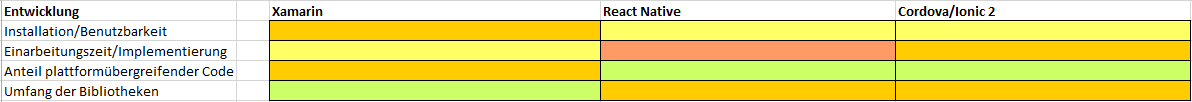
\includegraphics[width=1\textwidth]{Bilder/Auswertung_Entwicklung.PNG}
	\caption{Bewertungsmatrix Kategorie Entwicklung}
	\label{fig:AuswEntw}
\end{figure}

Hat man bereits ein Visual Studio installiert und möchte Xamarin integrieren, so ist dies nicht ohne Mehraufwand möglich. Einfacher ist es, Visual Studio direkt zusammen mit Xamarin zu installieren. Hierzu muss nur der Installer von der Xamarin Homepage heruntergeladen und ausgeführt werden. Alles Notwendige für die Entwicklung mit Xamarin ist bei der Installation von Visual Studio bereits vorausgewählt. Der Xamarin Installer installiert zusätzlich noch weitere benötigte Komponenten, wie ein Android SDK und NDK. Es muss keine weitere Software separat beschafft werden. Startet man nach der erfolgreichen Installation die IDE Visual Studio, so kann direkt mit der Entwicklung mit Xamarin gestartet werden, indem ein neues Projekt 'Android App' angelegt wird. Anders als bei der nativen Entwicklung mit Android Studio gibt es hier allerdings keine Design-Vorauswahl bei der Projekterstellung wie zum Beispiel einen \textit{NavigationDrawer} für die Navigation. Dafür gibt es sogenannte 'Pre Built Apps', das sind beispielhafte fertige Anwendungen, wie Shopping- oder CRM-Anwendungen.



\section{Hersteller}

\section{OS-Versionen}

\section{Funktionsumfang}

\section{GUI-Design}

\section{Interoperabilität}

\section{Tests}

\section{Performance}

\section{Programmiersprache}

\section{Sicherheit}
